\item A vertical pole is $100$ metres high. Find the angle subtended by the pole at a point on
the ground $100 \sqrt{3}$ meters from the base of the pole.

    \hfill\brak{10, 2021}\item The angle of elevation of the top of a tower from a point is found to be $60\degree$.At a point $40$ m above the first point, the angle of elevation of the top of the tower is $45\degree$.Find the height of the tower.
    \hfill\brak{10, 2021}\item A statue $1.6$m tall stands on the top of a pedestal. From a point on the ground, the angle of elevation of the top of statue is $60\degree$ and from the same point, the angle of elevation of the top of the pedestal is $45\degree$.Find the height of the pedestal.
    \hfill\brak{10, 2021}\item Two poles, $6$m and $11$ m high, stand vertically on the ground. If the distance between their feet is $12$ m, find the distance between their tops.
\end{enumerate}

	\hfill\brak{10, 2021}\item The angle of elevation of the top of a tower from a point on the ground,which is $30$ m away from the foot of the tower is $45\degree$ .What is the height of the tower ?
	\hfill\brak{10, 2021}\item Find the sun's altitude if the shadow of a 15 m high tower is ${15}\sqrt{3}$ m.
	\hfill\brak{10, 2021}\item From a point on the ground, $20$ m away from the foot of vertical tower, the angle of elevation of the top of the tower is $60\degree$. Find the height of the tower.
			\hfill\brak{10, 2021}\item In $\triangle$ $ABC$, $AB = {4\sqrt{3}}$ cm, $AC = 8 cm$ and $BC = 4 cm$. The angle $B$ is
				\begin{enumerate}
					\hfill\brak{10, 2021}\item $120\degree$
					\hfill\brak{10, 2021}\item $90\degree$
					\hfill\brak{10, 2021}\item $60\degree$
					\hfill\brak{10, 2021}\item $45\degree$
				\end{enumerate}
		\end{enumerate}
	\hfill\brak{10, 2021}\item To explain how trignometry can be used measure the height of an inaccessible object, a teacher gave the following example to students :

		A TV tower stands vertically n the bank of a canal. From a point on the other bank direct opposite the tower, the angle of the elevation of the top of the tower is $60\degree$.From another point 20 m away from this point to the foot of the tower, the angle of elevation of the top of the tower is $30\degree$ (as shown in Figure 1).

		\begin{figure}[h]
			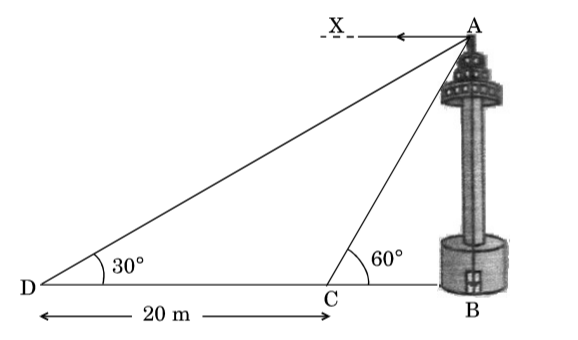
\includegraphics[width=\columnwidth]{cbse-math/figs/Problem.png}
			\caption{Projection of Tower}
			\label{fig:traingle}
		\end{figure}
		Based on the above, answer the following questions :
		\begin{enumerate}
			\item The width of the canal is
				\begin{enumerate}
					\hfill\brak{10, 2021}\item ${10}\sqrt{3} m$
					\hfill\brak{10, 2021}\item ${20}\sqrt{3} m$
					\hfill\brak{10, 2021}\item $10 m$
					\hfill\brak{10, 2021}\item $20 m$
				\end{enumerate}
			\item Height of the tower is
				\begin{enumerate}
					\hfill\brak{10, 2021}\item ${10}\sqrt{3} m$
					\hfill\brak{10, 2021}\item $10 m$
					\hfill\brak{10, 2021}\item ${20}\sqrt{3} m$
					\hfill\brak{10, 2021}\item $20 m$
				\end{enumerate}
			\item Distance of the foot of the tower from the point $D$ is
				\begin{enumerate}
					\hfill\brak{10, 2021}\item $20 m$
					\hfill\brak{10, 2021}\item $30 m$
					\hfill\brak{10, 2021}\item $10 m$
					\hfill\brak{10, 2021}\item ${20}\sqrt{3} m$
				\end{enumerate}
\hfill\brak{10, 2021}
